%&pdflatex

\documentclass[12pt]{article}

\usepackage[spanish, es-tabla]{babel}
\usepackage{enumerate}
\usepackage{lscape}
\usepackage{vmargin}
\usepackage{pdfpages}
\usepackage{fancyhdr}
\usepackage{graphicx}
\usepackage{float}
\usepackage{titlesec}
\usepackage[bottom]{footmisc}
\usepackage[hidelinks]{hyperref}
\usepackage{listings}
\usepackage{color}
\usepackage{colortbl}
\usepackage{xcolor}
\usepackage{amsmath}
\usepackage{array}
\usepackage{svg}
\usepackage{pgfgantt}
\usepackage[T1]{fontenc}
\usepackage[sfdefault]{AlegreyaSans} %% Option 'black' gives heavier bold face
%% The 'sfdefault' option to make the base font sans serif
\renewcommand*\oldstylenums[1]{{\AlegreyaSansOsF #1}}


%*******************************************************************************
\extrarowheight = -0.3ex
\renewcommand{\arraystretch}{2.25}
\setpapersize{A4}
\hypersetup{
    colorlinks=true,
    linkcolor=blue,
    urlcolor=purple,
    citecolor=black, 
    linktocpage=true,
}
\definecolor{gray95}{gray}{.95}
\definecolor{gray75}{gray}{.75}
\definecolor{barblue}{RGB}{153,204,254}
\definecolor{groupblue}{RGB}{51,102,254}
\definecolor{linkred}{RGB}{165,0,33}
\lstset{
    frame=Ltb,
    framerule=0pt,
     aboveskip=0.5cm,
     framextopmargin=3pt,
     framexbottommargin=3pt,
     framexleftmargin=0.4cm,
     framesep=0pt,
     rulesep=.4pt,
     backgroundcolor=\color{gray95},
     rulesepcolor=\color{cyan},
     %
     stringstyle=\ttfamily,
     showstringspaces = false,
     basicstyle=\small\ttfamily,
     commentstyle=\color{cyan},
     keywordstyle=\bfseries\color{purple},
     %
     numbers=left,
     numbersep=15pt,
     numberstyle=\small,
     numberfirstline = false,
     breaklines=true,
}

%minimizar fragmentado de listados
\lstnewenvironment{listing}[1][]
   {\lstset{#1}\pagebreak[0]}{\pagebreak[0]}


\lstdefinestyle{C}
   {
       language=C++,
   }

\lstdefinestyle{python}
    {
        language=Python,
    }

\setcounter{secnumdepth}{4}
%*******************************************************************************
%   Adding a new level of section --> subsubsubsection
%******************************************************************************
\titleclass{\subsubsubsection}{straight}[\subsection]

\newcounter{subsubsubsection}[subsubsection]
\renewcommand\thesubsubsubsection{\thesubsubsection.\arabic{subsubsubsection}}
\renewcommand\theparagraph{\thesubsubsubsection.\arabic{paragraph}} % optional; useful if paragraphs are to be numbered

\titleformat{\subsubsubsection}
  {\normalfont\normalsize\bfseries}{\thesubsubsubsection}{1em}{}
\titlespacing*{\subsubsubsection}
{0pt}{3.25ex plus 1ex minus .2ex}{1.5ex plus .2ex}

\makeatletter
\renewcommand\paragraph{\@startsection{paragraph}{5}{\z@}%
  {3.25ex \@plus1ex \@minus.2ex}%
  {-1em}%
  {\normalfont\normalsize\bfseries}}
\renewcommand\subparagraph{\@startsection{subparagraph}{6}{\parindent}%
  {3.25ex \@plus1ex \@minus .2ex}%
  {-1em}%
  {\normalfont\normalsize\bfseries}}
\def\toclevel@subsubsubsection{4}
\def\toclevel@paragraph{5}
\def\toclevel@paragraph{6}
\def\l@subsubsubsection{\@dottedtocline{4}{7em}{4em}}
\def\l@paragraph{\@dottedtocline{5}{10em}{5em}}
\def\l@subparagraph{\@dottedtocline{6}{14em}{6em}}
\makeatother

\setcounter{secnumdepth}{4}
\setcounter{tocdepth}{4}

%*****************************************************************************

\begin{document}

  \begin{titlepage}
    \centering
   {\bfseries\Large Universidad Carlos III de Madrid \par}
    \vspace{5cm}
    {\scshape\Huge Informe de la tercera práctica de laboratorio\par}
    \vspace{2cm}
    {\itshape\Large Diseño de circuitos electrónicos para comunicaciones}
    \vfill
    {\Large Autores: \par}
    \vspace{1cm}
    {\Large Markel Serrano y Daniel Theran}
    \vfill
    {\Large 19 de diciembre del 2022 \par}
  \end{titlepage}

  \section{Apartado 1: cálculos teóricos}

    \paragraph*{}
  
    
  \section{Apartado 2: resultados experimentales}

  \paragraph*{}
  Una vez realizado el montaje del circuito tal y como se indica en el informe, se obtienen, tomando los valores con el osciloscopio tal y como se indica en el informe, para un margen de fijado de 1.32 a 3.29 kHz de frecuencia
  de referencia, los siguientes valores para la salida en frecuencia de VCO, la amplitud de dicha señal y el desfase entre ambas:

\vspace*{1.0cm}

    \begin{table}[H]
      \begin{center}
          \begin{tabular}{| c | c | c | c |}
              \hline
              \rowcolor{black}
              \textcolor{white}{$F_{ref}$ (kHz)} & \textcolor{white}{$F_{VCO}$ (kHz)} & \textcolor{white}{$\Delta \phi$ ($\mu$ s)} & \textcolor{white}{$V_{VCO}$ (V)}\\ \hline
              1.11 & 15.6 & 172 &  2.12\\ \hline
              1.511 & 23.8 & 144 &  2.35\\ \hline
              1.911 & 29.4 & 124 &  2.61\\ \hline
              2.36 & 35.7 & 114 & 2.91\\ \hline
              2.901 & 41.7 & 102 &  3.27\\ \hline
              3.142 & 47.2 & 100 & 3.44\\ 
              \hline 
          \end{tabular}
          \caption{Tabla de resultados reales de la práctica}
          \label{tab:resul_r}
      \end{center}
    \end{table}

  \paragraph*{}
    A muestra de ejemplo, se han tomado como muestra para el informe las frecuencias de referencia de 1.11 kHz y 2.36 kHz, para las que se obtiene
    las siguientes señales de entrada y salida:

    \begin{figure}[H]
      \centering
      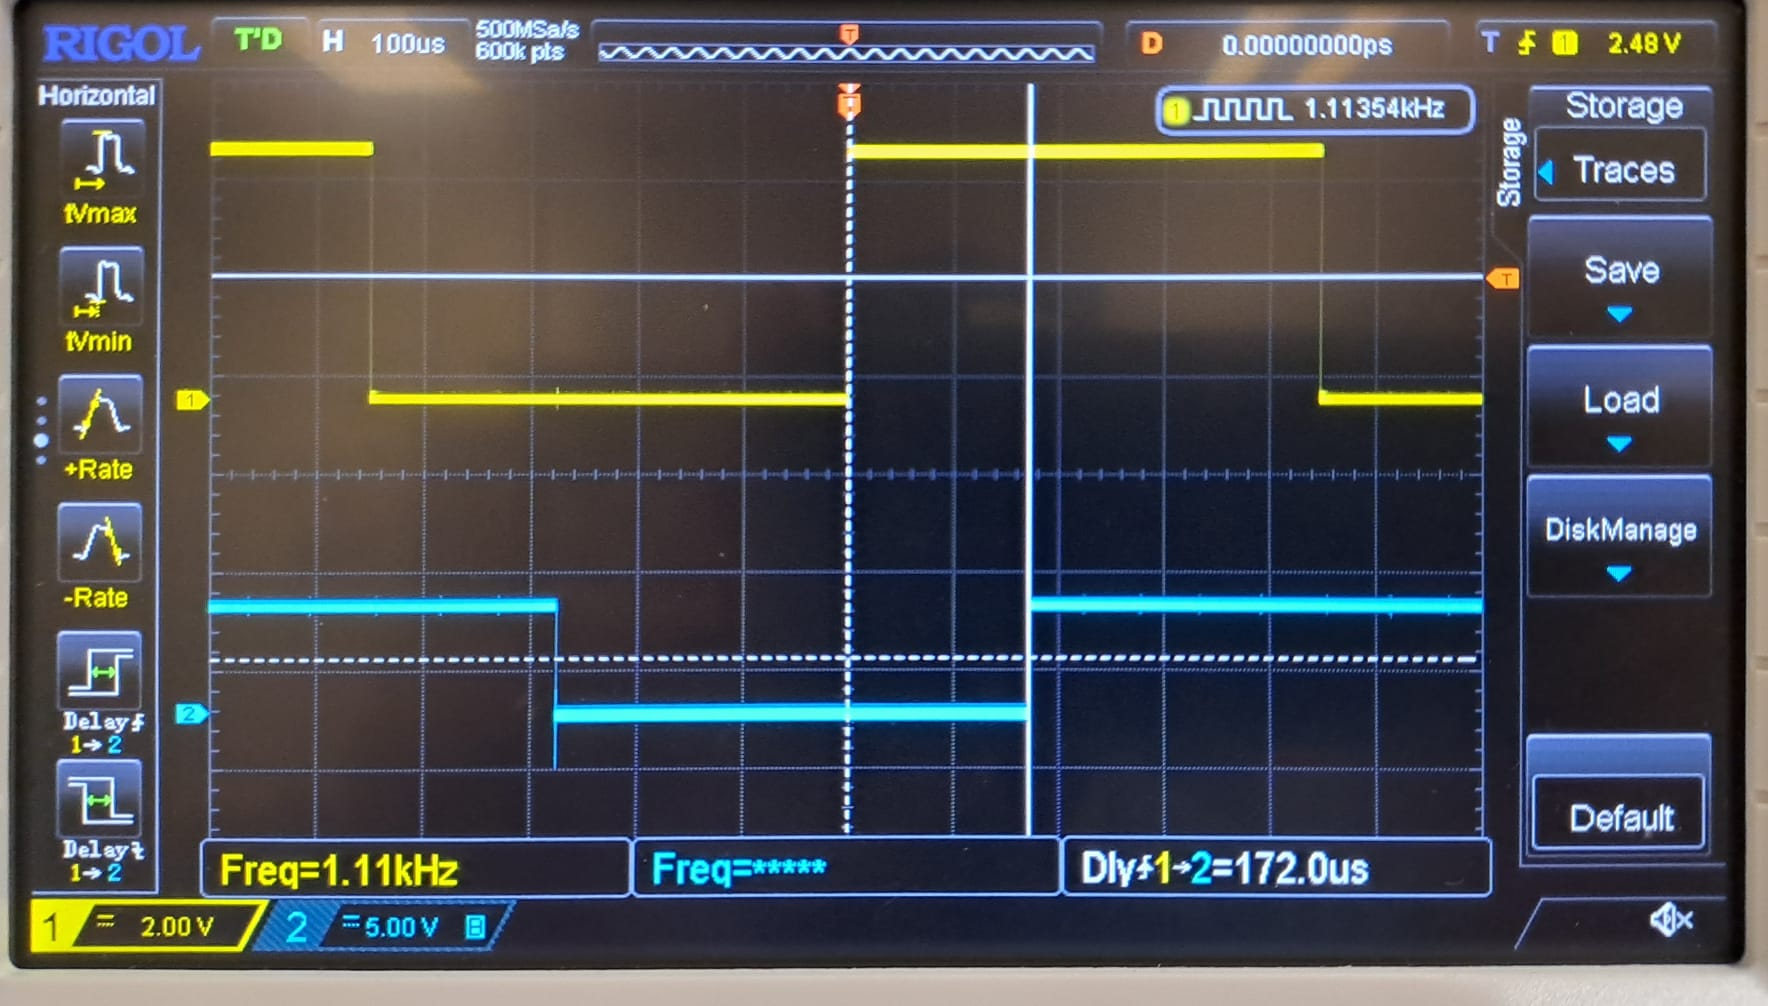
\includegraphics[width=1\linewidth]{img/1khz.jpeg}
      \caption{Señales para 1.11 kHz}%
      \label{fig:1khz}
    \end{figure}
    \paragraph*{}
   
    \begin{figure}[H]
      \centering
      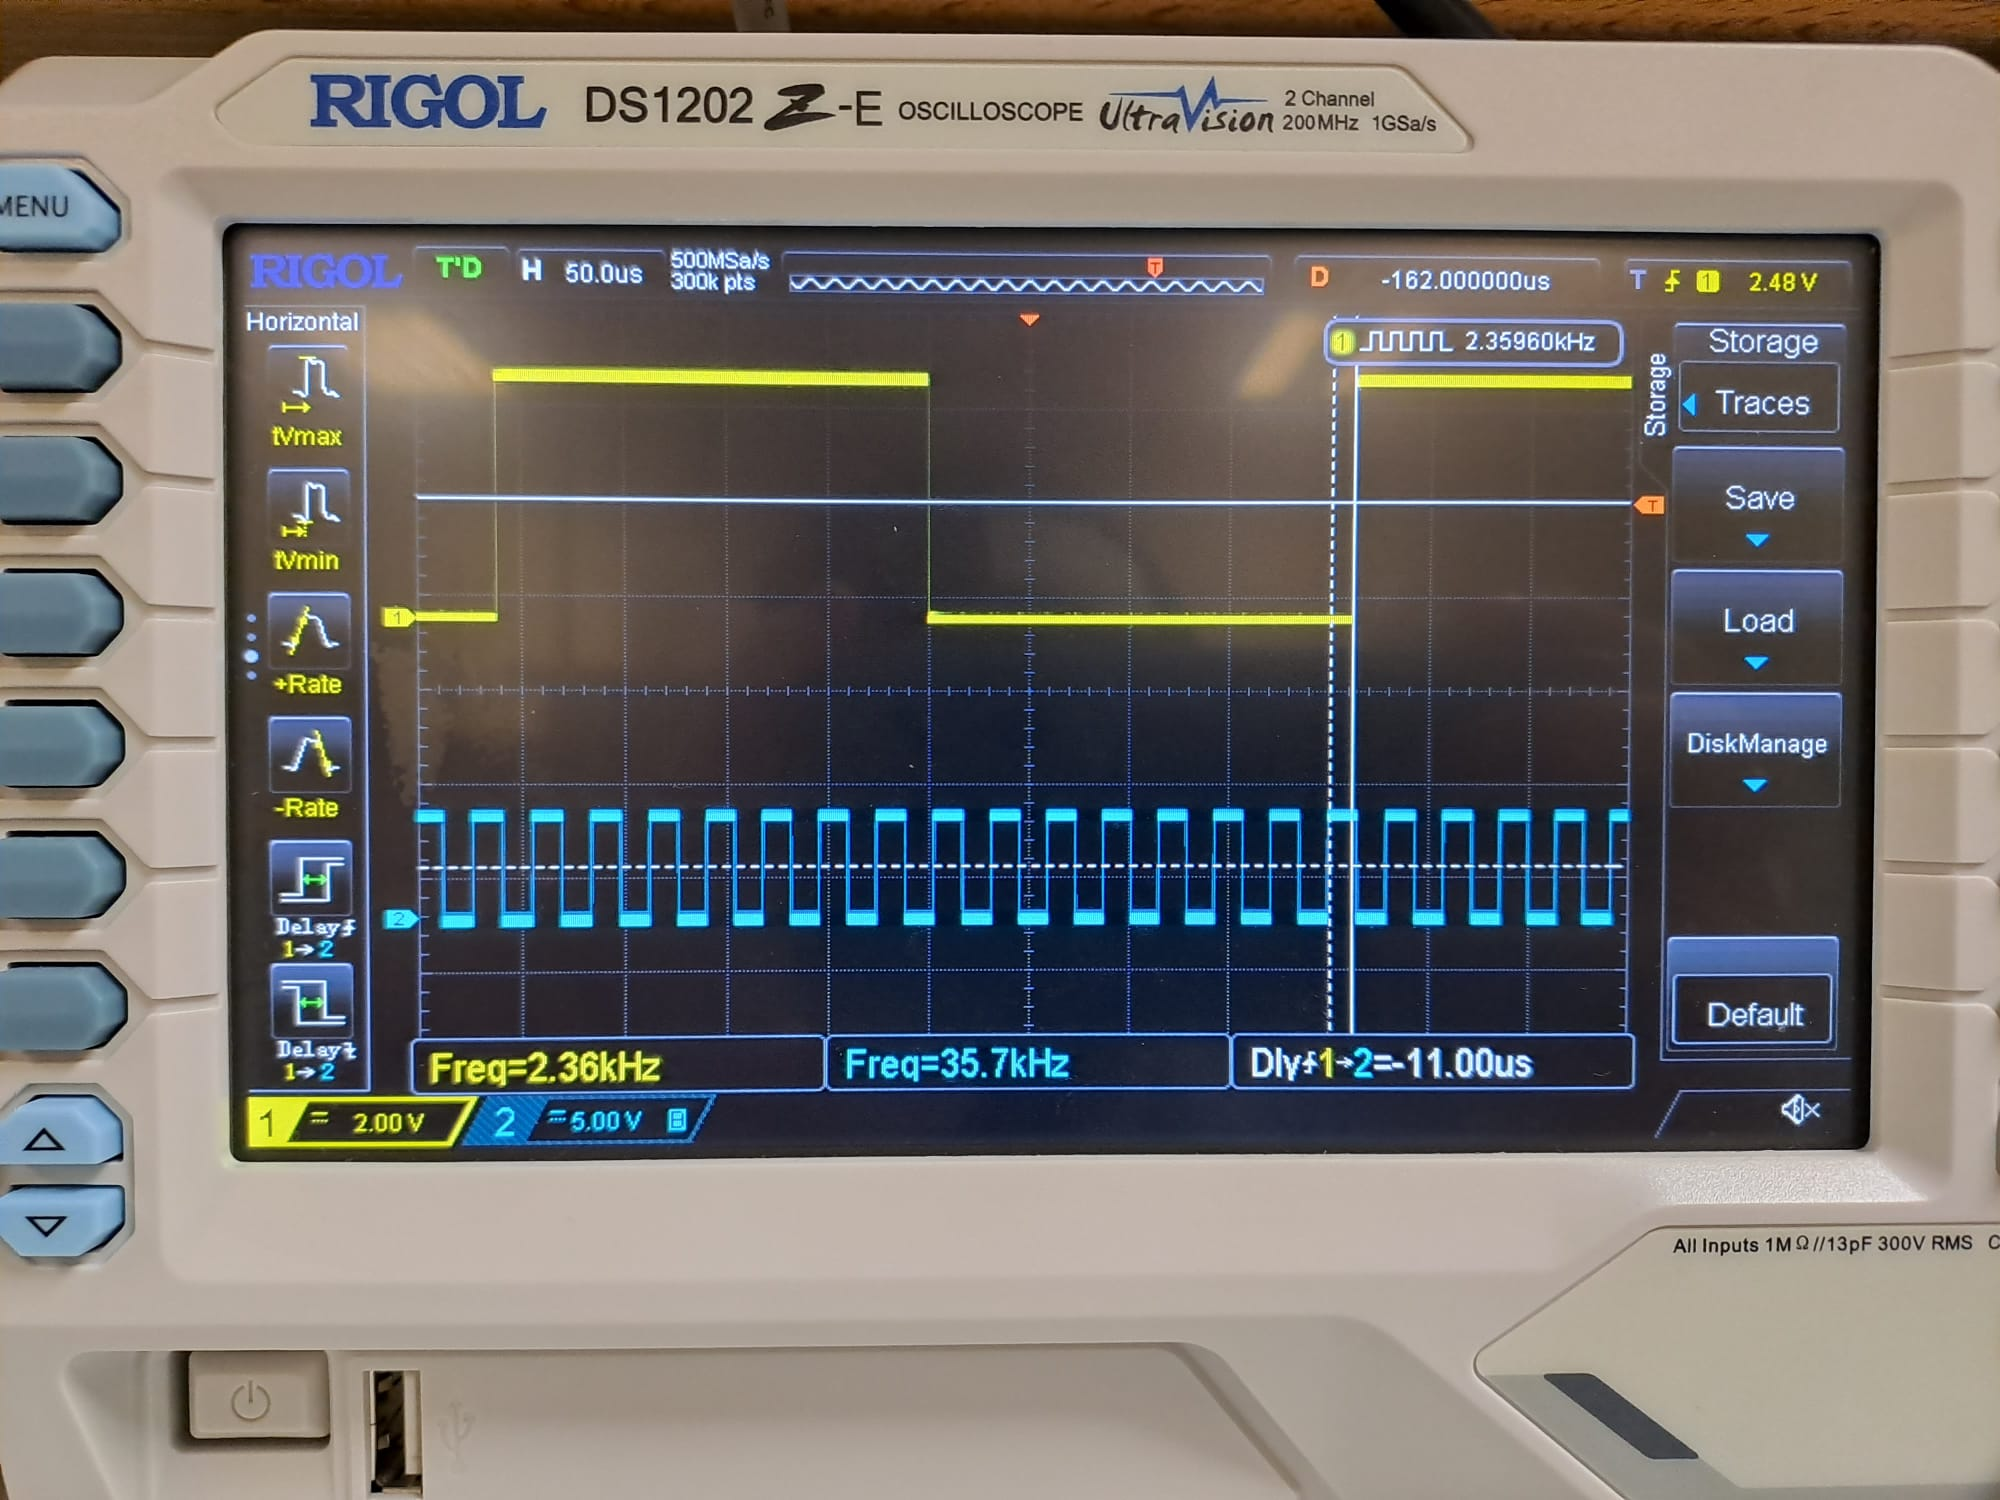
\includegraphics[width=1\linewidth]{img/2khz.jpeg}
      \caption{Señales para 2.36 kHz}%
      \label{fig:2khz}
    \end{figure}


    \paragraph*{}
   Una vez medidos los anteriores valores, podemos situar los distintos puntos encontrados para medir en dos gráficas distintas la frecuencia de salida VCO frente
   a la tensión VCO y la gráfica característica del detecor de fase, que muestra la relación entre las dos señales de entrada y de salida (es decir, el desfase entre ambas)
   y la ganancia en tensión que introduce el circuito, es decir, la tensión VCO.
    

    \begin{figure}[H]
      \centering
      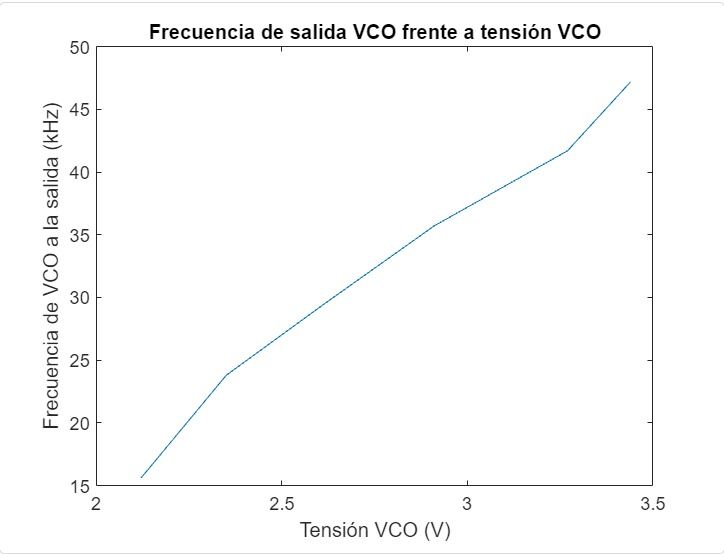
\includegraphics[width=1\linewidth]{img/grafica1.jpeg}
      \caption{Gráfica de relación entre frecuencia VCO y tensión VCO}%
      \label{fig:grafica1}
    \end{figure}

    \paragraph*{}
    Esta primera gráfica muestra la relación entre la frecuencia introducida por el circuito y la amplitud correspondiente. Por tanto, la pendiente de la recta obtenida
para esta gráfica nos muestra la ganancia en frecuencia introducida por el circuito. Así, mediante la ecuación:

 % \paragraph*{}
  \begin{center}
    $K_{VCO} = \frac{F_{VCO2} - F_{VCO1}}{V_{VCO2} - V_{VCO1}}$
  \end{center}
    
 % \paragraph*{}
  Obtenemos una ganancia de frecuencia de 19.45. Hay que remarcar que, debido a los errores de medición y a que la recta no ha sido representada estadísticamente sino como
  una gráfica que une los puntos obtenidos,
  el error en el cálculo de la pendiente es de una magnitud notable.

    \begin{figure}[H]
      \centering
      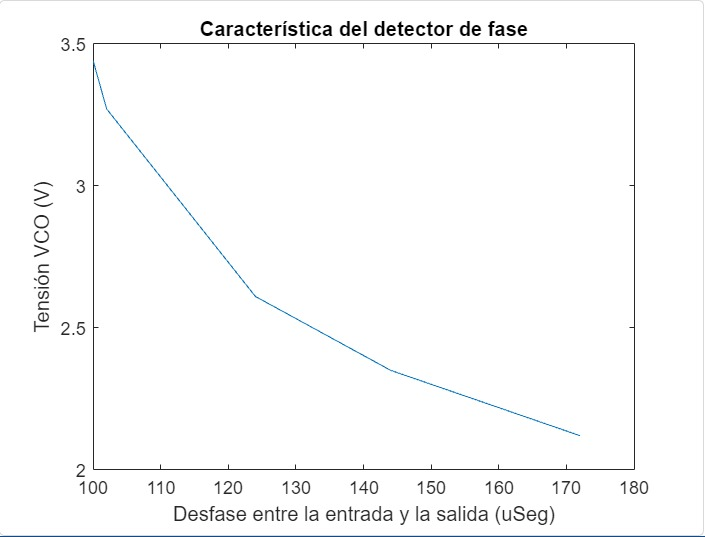
\includegraphics[width=1\linewidth]{img/grafica2.jpeg}
      \caption{Gráfica característica del detector de fase}%
      \label{fig:grafica2}
    \end{figure}
    
    \paragraph*{}
    La segunda gráfica muestra la relación entre la amplitud introducida por el circuito y los desfases entre la señal de entrada y salida. Por tanto, la pendiente de la recta obtenida
para esta gráfica nos muestra la característica del detector de fase. Así, mediante la ecuación:

 % \paragraph*{}
  \begin{center}
    $K_{CF} = \frac{V_{VCO2} - V_{VCO1}}{\Delta\phi_{2} - \Delta\phi_{1}}$
  \end{center}
    
 % \paragraph*{}
  Obtenemos una magnitud característica de $\frac{9.9}{\pi}$ V/rad, tomando el desfase, que en la tabla aparece representado en microsegundos, en radianes. Debe señalarse que se cometen los mismos errores en el cálculo que para el anterior caso.

    \section{Apartado 3: resultados conclusiones}

    


\end{document}